\section{Results}

\begin{figure*}[ht]
  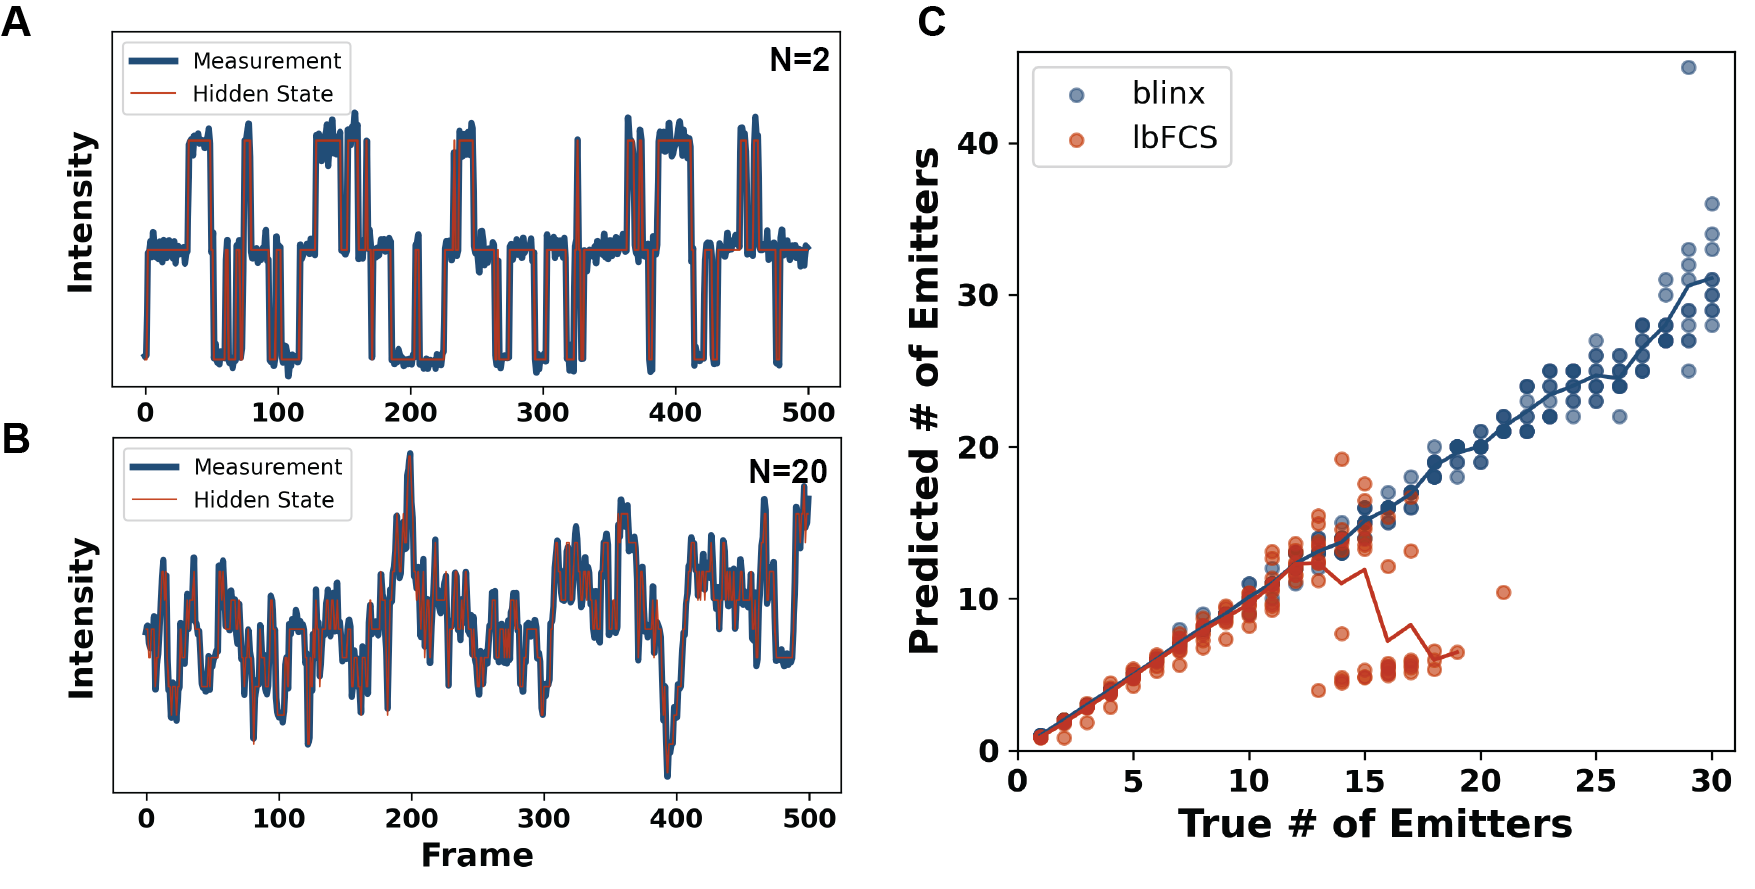
\includegraphics[width=\linewidth]{figures/comparison_lbfcs}
  \caption{A), B) simulated traces of 2 and 20 emitters respectively, generated with experimentally plausible parameters. C) Comparison of counting results between \ours and \lbfcs. Both models were applied to 10 simulated traces for each \truen. The accuracy of \lbfcs decreased significantly once \truen \textgreater 12 and failed completely for \truen \textgreater 21, while \ours was able to count up to \truen = 30.  }
  \label{fig:results:comparison}
\end{figure*}

\begin{figure}[ht]
  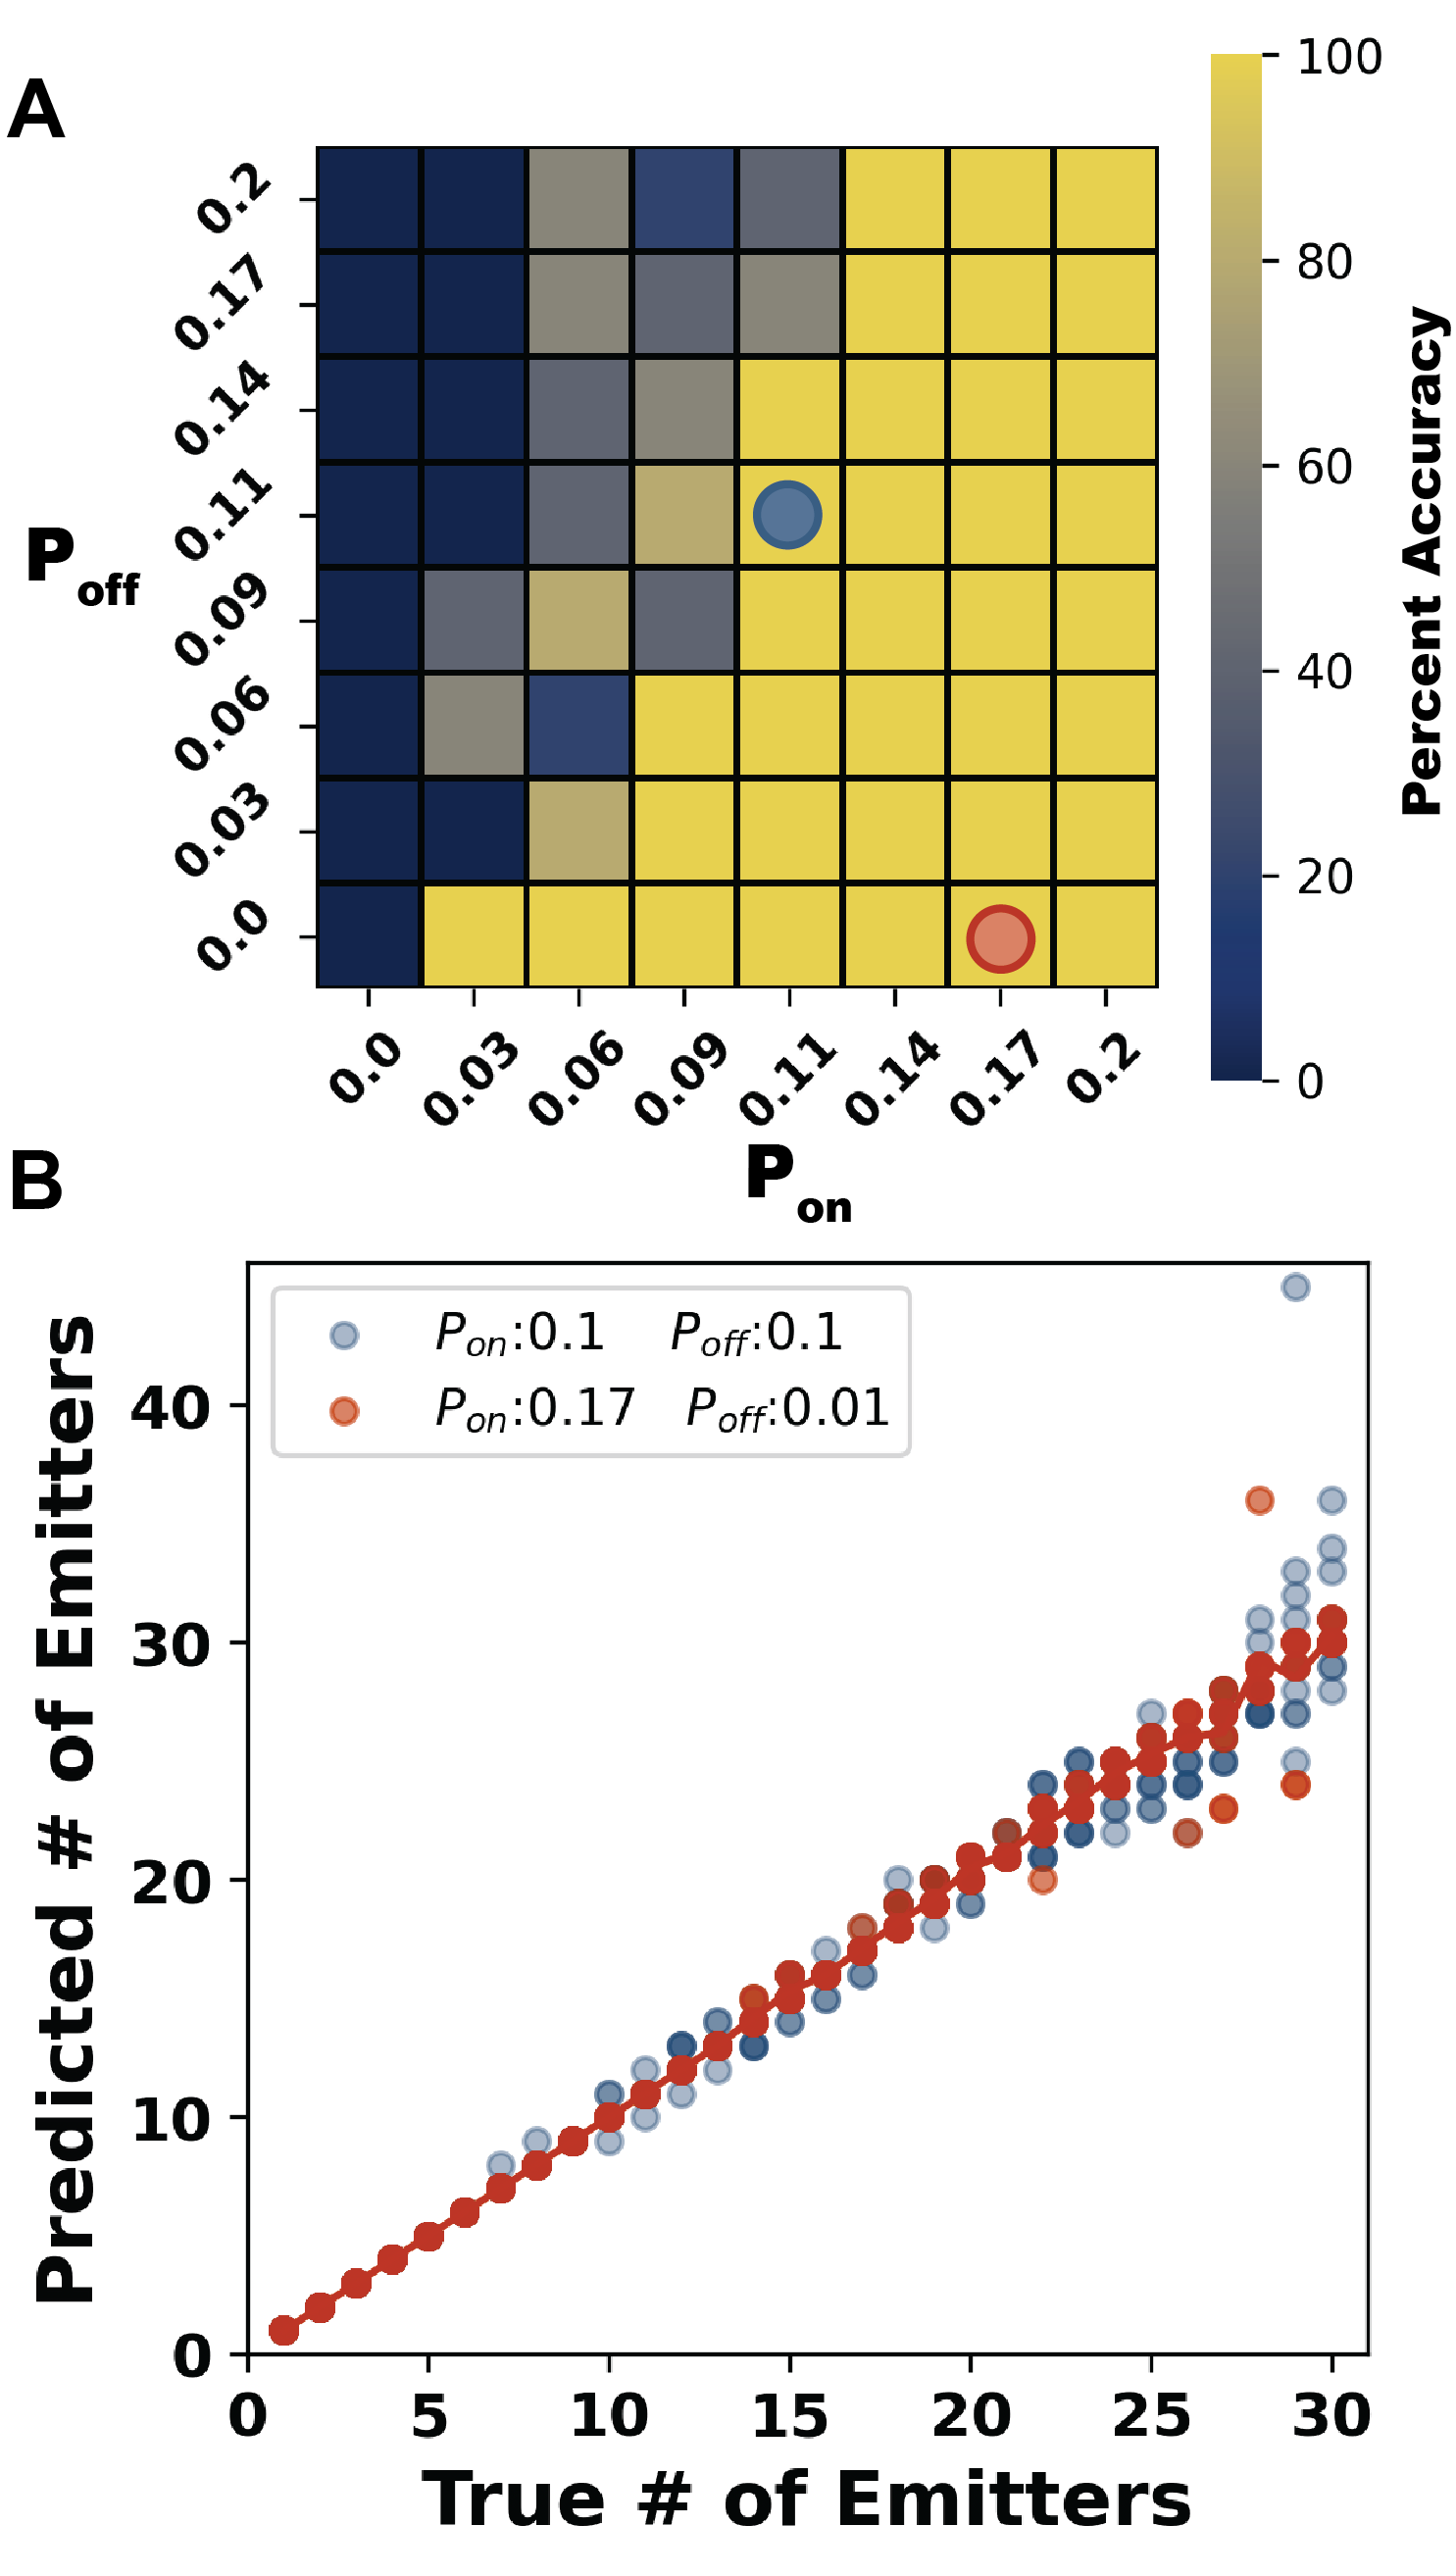
\includegraphics[width=\linewidth]{figures/kinetic_regime}
  \caption{A) The effect of rate parameters \pon and \poff on accuracy of \ours. All traces simulated traces with a \truen = 5.  Two points were then expanded to include \truen from one to 30 and an increase in accuracy was seen as \pon became greater than \poff. }
  \label{fig:results:regime}
\end{figure}

\subsection{Comparison to state of the art \lbfcs}

%
Over time, the intensity contributions from independent emitters, combined for each timepoint, produce a fluctuating intensity trace.
	%
	For a small number of emitters \ie $\truen = 2$, this trace contains series of easily distinguishable intensity steps corresponding to the number of emitters bound at each timepoint.
	%
	However, for a larger number of emitters \ie $\truen = 20$ individual intensity steps can no longer be distinguished \figref{fig:results:comparison}.

The current state of the art \lbfcs, was benchmarked on simulated traces of a known number of emitters up to $\truen = 30$, with experimentally plausible parameters $(\mu=2000, \sigma=0.03, \pon=0.1, \poff=0.1)$.
	%
	A direct comparison to other models is not possible due to differences in the types of data required.
	% 
	While \lbfcs performed well for \truen \textless 12, performance quickly declined with increasing \truen ultimately failing to produce any prediction for \truen \textgreater 21 \figref{fig:results:comparison}.
	% lbfcs is limited by histogram fitting of mu
	This drop in performance is a result of \lbfcs’s ability to identify the intensity of a single emitter ($\mu$ in \ours). \lbfcs is reliant on a histogram based method that works by identifying the specific $\y=1$ peak. However, for large \truen, observing this specific state becomes increasingly less likely. 

Holistic methods like \ours on the other hand, allow inferring the intensity of a single emitter
jointly with the number of emitters active at every time-step, thus
circumventing the problem of having to observe a specific number of active emitters.
% blinx performance 
	As a result \ours is able to count up to \truen = 30, effectively doubling the range of countable emitters \figref{fig:results:comparison}.

% summary and transition 


\subsection{Informing experiment}

% Transition to effect of parameters on model accuracy
Next we investigated the robustness of \ours to the underlying blinking rates of individual emitters. 
% maximize signal to noise through microscope parameters
To determine the role of blinking rates on the accuracy of \ours, traces were simulated with \truen = 5 and \pon and \poff ranging from 0.01 to 0.2 \figref{fig:results:regime}. 
% 3 regions in plot on>off on=off on<off
The results of these simulations are correlated within 3 distinct regimes: \poff \textgreater \pon, \poff = \pon, and \poff \textless \pon. 
% on<off
In the regime where \poff \textgreater \pon, \ours displayed a very low accuracy. This poor performance is related to the hidden state \y{t} observed at each timepoint. 
%
As \poff increases relative to \pon the likelihood of observing \y{t}=0 increases while the likelihood for observing any other state decreases. As a result, no matter the \truen, observed intensity traces in this regime only exhibit a small subset of the total possible states \y{}, leaving the model unable to determine \truen. 
%on=off
Interestingly, in the regime of \poff=\pon, an increase in \ours accuracy with increasing \pon is observed. Intuitively this makes sense, as both \pon and \poff increase transitions between states are observed more frequently, providing more information for the model to fit. This result also suggests that if the observation time were increased, the accuracy of all regimes would increase as well. 
%on>off

Based on these results, it was hypothesized that accuracy could be further
increased by shifting the experimental kinetics such that \pon $\gg$ poff. Simulating
traces with \pon=0.17 and \poff= 0.01, a significantly tighter distribution
around the correct count is observed, compared to traces simulated with pon =
poff = 0.1 \figref{fig:results:regime}. While it is not always possible to know the blinking
kinetics ahead of time, this finding can be used in experimental design, so as
to engineer a system so that pon \textgreater   poff and the counting potential of the model
is maximized.
